\documentclass{article}
\usepackage{amsmath}
\usepackage{amssymb}
\usepackage{graphicx}
\usepackage{hyperref}
\usepackage[version=4]{mhchem}


\begin{document}
\section*{Problem}
In \(\triangle A B C, \angle B=2 \angle A\) and \(A B=2 B C\). Show that \(A B^{2}=A C^{2}+B C^{2}\).\\
\centering
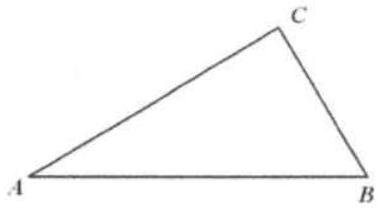
\includegraphics[width=\textwidth]{images/016.jpg}

\section*{Solution}
(D).\\
Method 1 (official solution):\\
\centering
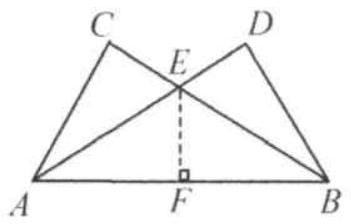
\includegraphics[width=\textwidth]{images/093(2).jpg}


In the adjoining figure \(M V\) is an altitude of \(\triangle A M V\) ( \(30^{\circ}-60^{\circ}-90^{\circ}\) triangle), and \(M V\) has length \(2 \sqrt{3}\). The required area of triangle \(A B V\) is \(\frac{1}{2}(A B)(M V)\)\\
\(=\frac{1}{2} \times 12 \times 2 \sqrt{3}=12 \sqrt{3}\).

Method 2 (our solution):\\
In the adjoining figure we draw \(E F\), an altitude of \(\triangle A E B\). \(E F\) divides the figure into four congruent triangles. Since \(\triangle A B C\) is a \(30^{\circ}-60^{\circ}-90^{\circ}\) triangle, thus \(A B=\) \(12, A C=6\) and \(B C=6 \sqrt{3}\). The area of \(\triangle A B C\) is \(\frac{1}{2}(A C)(B C)=\frac{1}{2} \times 6 \times 6 \sqrt{3}\) \(=18 \sqrt{3}\).\\
The required area of triangle \(A B E\), therefore is \(\frac{2}{3} \times 18 \sqrt{3}=12 \sqrt{3}\).

\end{document}
